%de https://tex.stackexchange.com/questions/427792/specification-mask-of-a-filter
\documentclass[border=5mm]{standalone}
\usepackage{tikz}
\usetikzlibrary{patterns,calc}
\begin{document}
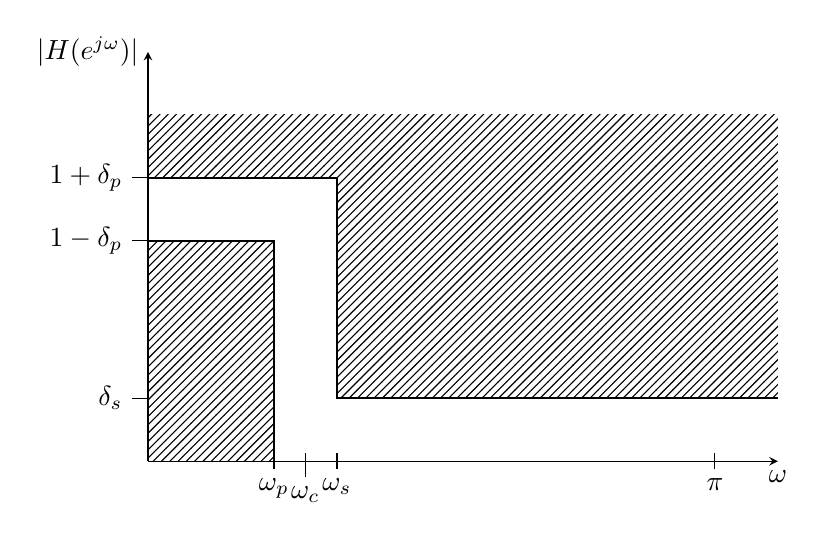
\begin{tikzpicture}[x=8cm,y=4cm]
	%\draw[step=0.5,help lines] (0,-1mm) grid (2mm,3mm);
  \draw[-stealth](0,0)--(1,0) node[below]{$\omega$};
	\draw[-stealth](0,0)--(0,1.3) node[left]{$|H(e^{j\omega})|$};
  \foreach \x/\y [count=\ind] in {0.2/0.7,0.25/0.7,0.3/0.9,0.3/0.2}{% Corners in the filter def
    \coordinate (Corner-\ind) at (\x,\y);
  }
	\coordinate (Corner-5) at (0.9,0.7);
  \path [pattern=north east lines](0,0) rectangle (Corner-1);
  \path [pattern=north east lines](0,1.1) rectangle (Corner-3);
	\path [pattern=north east lines](Corner-4) rectangle (1,1.1);%(Corner-4 |- {(1,1)});
  %\path [pattern=north east lines](Corner-4) rectangle (1,0);
  \draw[thick] (Corner-1 -| {(0,0)}) -| (Corner-1 |- {(0,0)});
	\draw[thick] (0,0.9) -- (Corner-3);%(Corner-1 -| {(0,0)}) -| (Corner-3 |- {(0,0)});
	\draw[thick] (Corner-3 |- {(0,0.9)}) -- (Corner-4) -- (1,0.2);%| (Corner-4 |- {(0,1)});
  %\draw[thick] (Corner-4 -| {(1,0)}) -| (Corner-4 |- {(1,0)});
  %% Draw tick marks
  \draw (Corner-1 |- {(0,1mm)}) -- +(0,-2mm) node[below]{$\omega_p$};
  \draw (Corner-2 |- {(0,1mm)}) -- +(0,-3mm) node[below]{$\omega_c$};
  \draw (Corner-4 |- {(0,1mm)}) -- +(0,-2mm) node[below]{$\omega_s$};
  \draw (Corner-5 |- {(0,1mm)}) -- +(0,-2mm) node[below]{$\pi$};
  %\draw (Corner-3 |- {(0,1mm)}) -- +(0,-2mm) node[below]{$\omega'_{p2}$};
  %\draw (Corner-4 |- {(0,1mm)}) -- +(0,-2mm) node[below]{$\omega'_{a2}$};
  \draw (Corner-1 -| {(0,1mm)}) -- +(-2mm,0) node[left]{$1-\delta_p$};
  \draw (Corner-4 -| {(0,1mm)}) -- +(-2mm,0) node[left]{$\delta_s$};
  \draw (Corner-3 -| {(0,1mm)}) -- +(-2mm,0) node[left]{$1+\delta_p$};
\end{tikzpicture}
\end{document}
